\section{Gaussian Processes}
\framecard{\insertsection}

\subsection{Recap}
\begin{frame}{\insertsubsection}
    \framesubtitle{Linear Regression} 

    \textcolor{UniGold}{\textbf{What was done until here?}}
    \begin{itemize}
        \item We assumed that our targets $t$ were \textcolor{UniOrange}{\textbf{i.i.d.}} and given by $t = y(\mathbf{x}) + \varepsilon$, where $\varepsilon \sim \mathcal{N}(0,\beta)$.
        \item Our model is given by $\mathbf{y}(\mathbf{x}) = \Phi^{\top} \mathbf{w}$, where $\Phi$ is the \textcolor{UniOrange}{\textbf{design matrix}}, and this caracterize our model as \textcolor{UniOrange}{\textbf{linear in parameters}}.
        \item The \textcolor{UniOrange}{\textbf{design matrix}} was defined as $ \phi_{i,j} = \phi_i(\mathbf{x}_j)$.
        \item The \textcolor{UniOrange}{\textbf{parameters}} were given by $\mathbf{w} = \left( \Phi^{\top} \Phi \right)^{-1}\Phi^{\top} \mathbf{t}$.
        \item These \textcolor{UniOrange}{\textbf{parameters}} calculated at the minimum of the cost function are called \textcolor{UniOrange}{\textbf{maximum likelihood}}.
    \end{itemize}
    \begin{columns}
        \begin{column}{0.5\linewidth}  
        \begin{center}
        \centering
        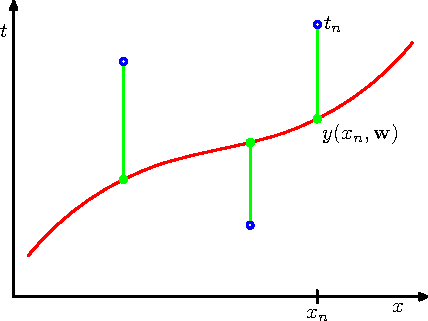
\includegraphics[width=0.9\linewidth]{Figure1c3.pdf}
         \end{center}
    \end{column}
    \begin{column}{0.5\linewidth}  %%<--- here
        \begin{figure}
            \setlength\fwidth{0.07\textwidth}
            \input{./codes/lnReg/"lnReg".tex}
        \end{figure}
    \end{column}
    \end{columns}

\end{frame}

\begin{frame}{\insertsubsection}
    \framesubtitle{Bayesian Linear Regression} 

    \textcolor{UniGold}{\textbf{What was done until here?}}
    \begin{itemize}
        \item We put an \textcolor{UniOrange}{\textbf{uncertainty}} over the targets $t$ and the parameters $\mathbf{w}$.
        \item We assumed that targets being \textcolor{UniOrange}{\textbf{distributed}} as $p( t| \mathbf{x}, \mathbf{w}, \beta) = \mathcal{N} ( t | y(\mathbf{x}, \mathbf{w}), \beta^{-1})$.
        \item By \textcolor{UniOrange}{\textbf{Bayes' Rule}} we obtained that $p\left( \mathbf{w} | \mathbf{x}, \mathbf{t}, \alpha, \beta \right) \propto p\left(  \mathbf{t} |\mathbf{w} ,\mathbf{x}, \beta \right) p\left( \mathbf{w} | \alpha \right)$
        \item This allowed to make an \textcolor{UniOrange}{\textbf{inference}} to obtain a \textcolor{UniOrange}{\textbf{prediction}} of the parameters in the \textcolor{UniOrange}{\textbf{weight-space}}.
        
    \end{itemize}

    % \begin{figure}
	% 	\label{fig:baReg}
    %     \hspace*{-1.4cm}\includegraphics[totalheight=0.3\textheight]{./codes/baReg/"baReg".eps}
	% \end{figure}
\end{frame}


\begin{frame}{\insertsubsection}
    \framesubtitle{A more clear way to se what is happening...} 

    % \textcolor{UniGold}{\textbf{A more clear way to se what is happening...}}

    % \begin{figure}
	% 	\label{fig:baReg}
    %     \hspace*{-1.4cm}\includegraphics[totalheight=0.3\textheight]{"baRegInfII".eps}
	% \end{figure}
\end{frame}

%%%%%%%%%%%%%%%%%%%%%%%%%%%%%%%%%%%%%%%%%%%%%%%%%%%%%%%%%%%%%%%%%%%%%%%%%%%%%%%%%%%%%%%%%%%%%

\begin{frame}{\insertsubsection}
    \framesubtitle{Introducing kernels}

    \textcolor{UniGold}{\textbf{What is kernel?}}
    \begin{equation*}
        \begin{aligned} f_{*} | \mathbf{x}_{*}, \Phi, \mathbf{t} & \sim \mathcal{N}\left(\boldsymbol{\phi}_{*}^{\top} \mathbf{S}_0 \Phi\left(K+\beta^{-2} I\right)^{-1} \mathbf{t}, \boldsymbol{\phi}_{*}^{\top} \mathbf{S}_0 \boldsymbol{\phi}_{*}-\boldsymbol{\phi}_{*}^{\top} \mathbf{S}_0 \Phi\left(K+\beta^{-2} I\right)^{-1} \Phi^{\top} \mathbf{S}_0 \boldsymbol{\phi}_{*}\right)
        \end{aligned}
    \end{equation*}

    \begin{itemize}
        \item We could observe the appearance of terms like $\Phi^{\top} \mathbf{S}_0 \Phi, \boldsymbol{\phi}_{*}^{\top} \mathbf{S}_0 \Phi, \text { or } \boldsymbol{\phi}_{*}^{\top} \mathbf{S}_0 \boldsymbol{\phi}_{*}$.
        \item The common term between these operations is $k(\mathbf{x},\mathbf{x^{\prime}}) = \boldsymbol{\phi}(\mathbf{x})^{\top} \mathbf{S}_0 \boldsymbol{\phi}\left(\mathbf{x}^{\prime}\right)$
        \item Then we define $k(\cdot,\cdot)$ as \textcolor{UniOrange}{\textbf{kernel function}}
        \item This technique is particularly valuable in situations where it is more convenient to compute the kernel than the design matrix vectors themselves.
        
    \end{itemize}
    
\end{frame}

%%%%%%%%%%%%%%%%%%%%%%%%%%%%%%%%%%%%%%%%%%%%%%%%%%%%%%%%%%%%%%%%%%%%%%%%%%%%%%%%
\subsection{Gaussian processes}
\begin{frame}{\insertsubsection}
    \framesubtitle{In change of space}

    \begin{itemize}
        \item Previously we make the inference in the \textcolor{UniOrange}{\textbf{feature-space}} and then we find the function distribution.
        \item Now we'll make the inference directly on \textcolor{UniOrange}{\textbf{function-space}}.
        \item Let's define
    \end{itemize}

    \begin{definition}
        \textit{
        A \textcolor{UniGold}{\textbf{Gaussian process}} is a collection of random variables which any finite number of them have a joint Gaussian distribution.}
    \end{definition}
\end{frame}

\begin{frame}{\insertsubsection}
    \framesubtitle{In change of space}

    \textcolor{UniGold}{\textbf{Mean and covariance function}}
    \begin{itemize}
        \item As the Gaussian distribution, the $\mathcal{GP}$ is characterized by its \textcolor{UniOrange}{\textbf{mean function}} $m(\mathbf{x})$ and its \textcolor{UniOrange}{\textbf{covariance function}} $k(\mathbf{x,x}^{\prime})$ of a real process $f(\mathbf{x})$.
    \item For a Gaussian processes
    \begin{equation*}
        f(\mathbf{x})  \sim \mathcal{G} \mathcal{P}\left(m(\mathbf{x}), k\left(\mathbf{x}, \mathbf{x}^{\prime}\right)\right)
    \end{equation*}
    \item We have
    \begin{equation*}
    \begin{aligned} m(\mathbf{x}) &=\mathbb{E}[f(\mathbf{x})] \\ k\left(\mathbf{x}, \mathbf{x}^{\prime}\right) &=\mathbb{E}\left[(f(\mathbf{x})-m(\mathbf{x}))\left(f\left(\mathbf{x}^{\prime}\right)-m\left(\mathbf{x}^{\prime}\right)\right)\right] \end{aligned}        
    \end{equation*}
    \end{itemize}
\end{frame}